
\begin{figure}
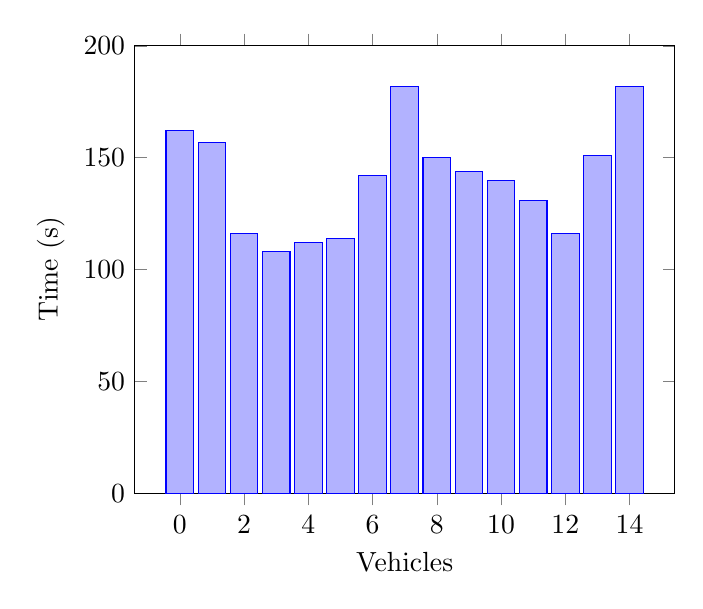
\begin{tikzpicture}
\begin{axis}[
legend style={anchor=west},
xlabel=Vehicles,
ylabel=Time (s),
ymin=0,
ybar,
]
\addplot coordinates {
(0, 162)
(1, 157)
(2, 116)
(3, 108)
(4, 112)
(5, 114)
(6, 142)
(7, 182)
(8, 150)
(9, 144)
(10, 140)
(11, 131)
(12, 116)
(13, 151)
(14, 182)
};

\end{axis}
\end{tikzpicture}
\label{tik:0:19_O, 19_O.-60, 17_N, 15_S, 15_S.-30, 13_N, 13_N.-40, 11_N, 8_N, 7_N, 7_N.-60, 5_N, 4_N, 4_N.-60, 3_O}
\caption{0 percent diving with GSC on route $19_O, 19_O.-60, 17_N, 15_S, 15_S.-30, 13_N, 13_N.-40, 11_N, 8_N, 7_N, 7_N.-60, 5_N, 4_N, 4_N.-60, 3_O$}
\end{figure}
